\documentclass[11pt,a4paper]{article}

\usepackage[utf8]{inputenc}
\usepackage[T1]{fontenc}
\usepackage{amsmath,amssymb,amsfonts}
\usepackage{physics}
\usepackage{hyperref}
\usepackage{booktabs}
\usepackage{geometry}
\usepackage{enumitem}
\usepackage{xcolor}
\usepackage{graphicx}
\usepackage{subcaption}

\geometry{margin=1in}
\hypersetup{colorlinks=true, linkcolor=blue, urlcolor=blue, citecolor=blue}

\title{Comparison of VQE, VQITE, and TTITE\\
  for Charmonium Spectroscopy\\[0.5em]
  \large Apples-to-Apples Benchmark on the Woloshyn Hamiltonian}

\author{quarkonium-simulations project}
\date{\today}

\begin{document}
\maketitle

\begin{abstract}
We compare three quantum-computing methods---the Variational Quantum
Eigensolver (VQE), Variational Quantum Imaginary-Time Evolution (VQITE),
and Trotter--Taylor Imaginary-Time Evolution (TTITE)---on the same
2-qubit charmonium Hamiltonian with spin-dependent interactions.
All three methods use the same direct qubit encoding and the same
physical parameters, enabling a controlled comparison of accuracy,
convergence speed, and noise sensitivity.
\end{abstract}

\tableofcontents
\newpage

%=============================================================================
\section{Setup}
%=============================================================================

\subsection{The Hamiltonian}

We use the Woloshyn charmonium Hamiltonian (arXiv:2301.10828v2), which
describes a charm--anticharm system with the Cornell potential plus a
spin-dependent contact term:
\begin{equation}
  V(r) = -\frac{a}{r} + b\,r + V_s(r)\,\vec{S}_c \cdot \vec{S}_{\bar{c}}
\end{equation}

The Hamiltonian is expanded in a harmonic oscillator basis truncated
to $N=4$ radial states, yielding a $4 \times 4$ matrix encoded on
\textbf{2 qubits} via direct state mapping:
$\ket{00} \leftrightarrow n\!=\!0$,
$\ket{01} \leftrightarrow n\!=\!1$,
$\ket{10} \leftrightarrow n\!=\!2$,
$\ket{11} \leftrightarrow n\!=\!3$.

Three spin channels are studied:
${}^1S_0$ ($\eta_c$, spin singlet),
${}^3S_1$ ($J/\psi$, spin triplet), and
${}^1P_1$ ($h_c$, $P$-wave singlet).

The Pauli decomposition of each channel has 10 terms:
\begin{equation}
  H = c_0\,II + c_1\,IZ + c_2\,ZI + c_3\,ZZ + c_4\,IX + c_5\,XI
    + c_6\,ZX + c_7\,XZ + c_8\,XX + c_9\,YY
\end{equation}

\subsection{The Three Methods}

\paragraph{VQE (Variational Quantum Eigensolver)}
Minimizes the energy expectation value over a parameterized ansatz:
\begin{equation}
  E(\vec{\theta}) = \mel{\psi(\vec{\theta})}{H}{\psi(\vec{\theta})} \geq E_0
\end{equation}
using the COBYLA classical optimizer. The ansatz is a 3-parameter
$R_Y$--CNOT circuit on 2 qubits.

\paragraph{VQITE (Variational Quantum Imaginary-Time Evolution)}
Evolves variational parameters along the imaginary-time gradient:
\begin{equation}
  \sum_j A_{ij}\,\dot{\theta}_j = C_i, \qquad
  C_i = -\frac{\partial E}{\partial\theta_i}, \quad
  A_{ij} = \text{Re}\!\left[\frac{\partial\bra{\psi}}{\partial\theta_i}
    \frac{\partial\ket{\psi}}{\partial\theta_j}\right]
\end{equation}
where $A$ is the quantum metric tensor. Uses the same 3-parameter ansatz
as VQE, with parameters updated via forward Euler.

\paragraph{TTITE (Trotter--Taylor Imaginary-Time Evolution)}
Implements imaginary-time evolution directly (no ansatz) via:
\begin{equation}
  e^{-H\tau} \approx \prod_{i=1}^m \left(\alpha_i\,I + \beta_i\,h_i\right)^L
\end{equation}
where $\alpha_i$ and $\beta_i$ are Taylor expansion coefficients and each
factor is applied via an ancilla-qubit Linear Combination of Unitaries (LCU)
circuit with postselection.

\subsection{Shared Ansatz}

All variational methods (VQE, VQITE) use the same hardware-efficient ansatz:
\begin{equation}
  \begin{aligned}
  &q_0: \quad R_Y(\theta_0) - \bullet - \\
  &q_1: \quad R_Y(\theta_1) - \oplus - R_Y(\theta_2)
  \end{aligned}
\end{equation}
With 3 parameters, this circuit spans all real superpositions of the 4 basis states.

%=============================================================================
\section{Noiseless Results}
%=============================================================================

\subsection{Ground-State Energy}


\begin{center}
\small
\begin{tabular}{@{}l l r r r r r@{}}
\toprule
Channel & Method & $E_0$ [fm$^{-1}$] & Exact & Error & Fidelity & Time [s] \\
\midrule
    1S0 & VQE & 0.3647 & 0.3913 & -0.026626 & 0.999505 & 18.63 \\
    1S0 & VQITE & 0.3855 & 0.3913 & -0.005793 & 0.999904 & 154.79 \\
    1S0 & TTITE & 0.3930 & 0.3913 & 0.001739 & 0.999835 & 0.82 \\
    \midrule
    3S1 & VQE & 0.8409 & 0.7522 & 0.088755 & 0.969828 & 20.43 \\
    3S1 & VQITE & 0.7341 & 0.7522 & -0.018092 & 0.999980 & 166.31 \\
    3S1 & TTITE & 0.7723 & 0.7522 & 0.020164 & 0.999892 & 0.99 \\
    \midrule
    1P1 & VQE & 2.7741 & 2.7813 & -0.007189 & 0.996685 & 15.56 \\
    1P1 & VQITE & 2.8124 & 2.7813 & 0.031096 & 0.982777 & 164.69 \\
    1P1 & TTITE & 2.7817 & 2.7813 & 0.000351 & 0.999978 & 0.88 \\
\bottomrule
\end{tabular}
\end{center}



\begin{figure}[htbp]
\centering
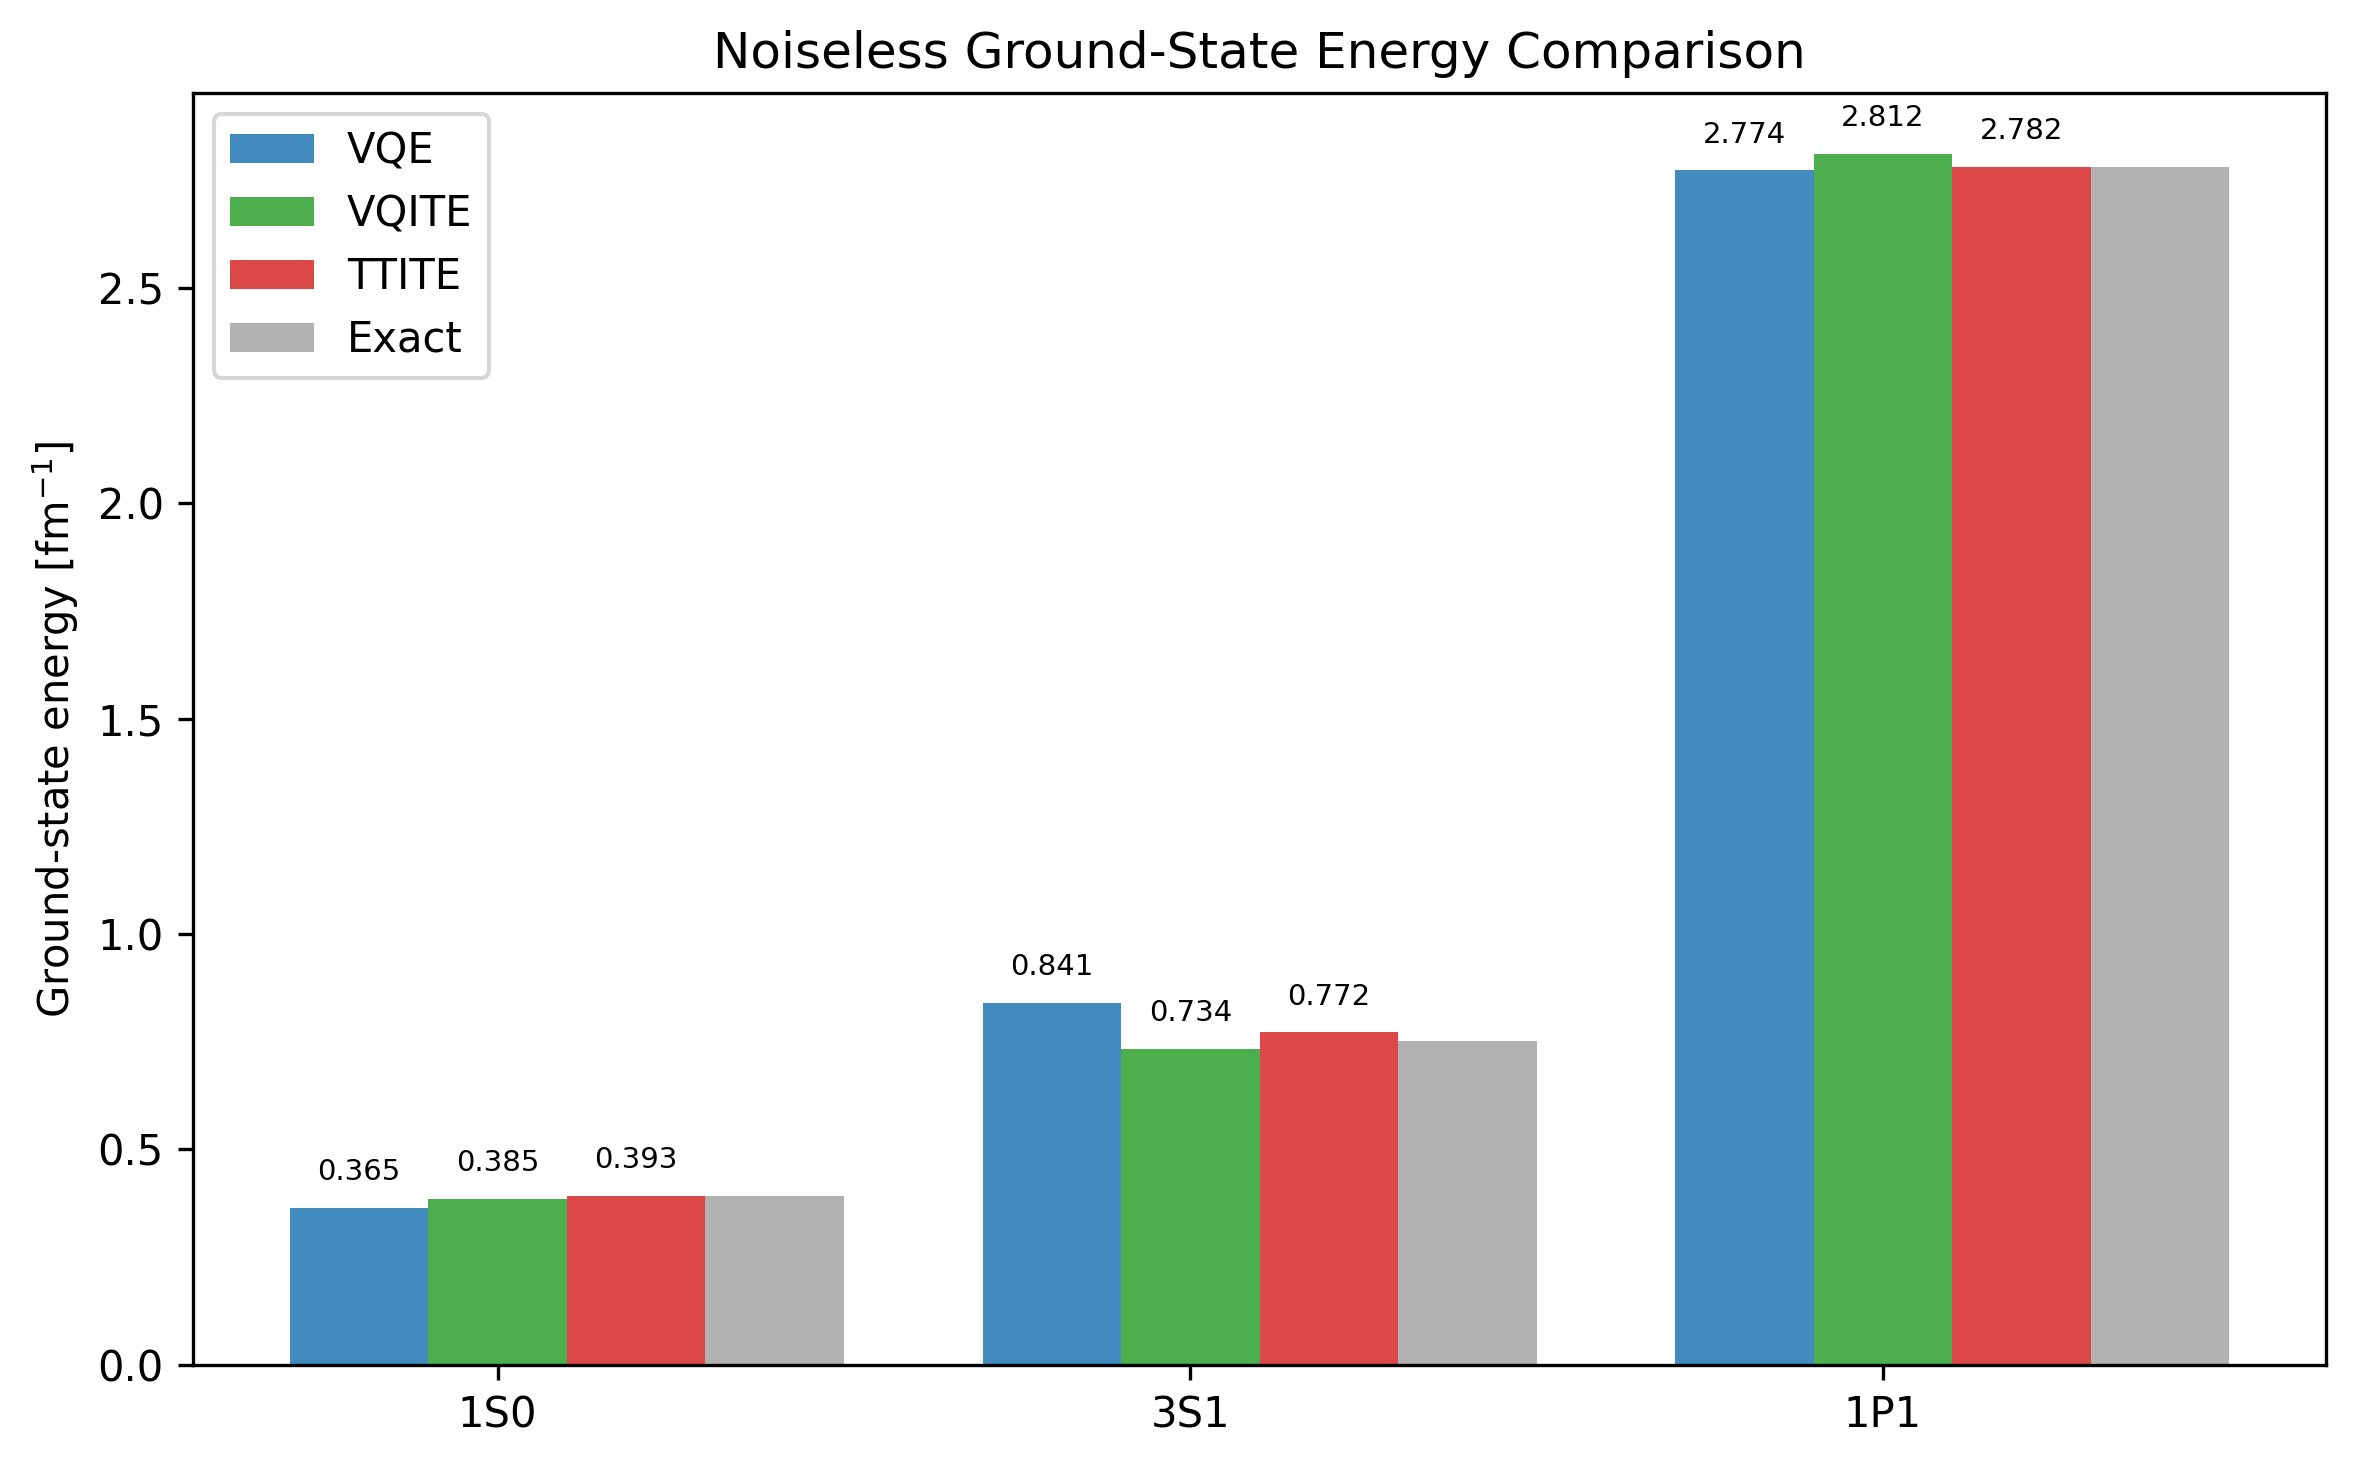
\includegraphics[width=0.85\textwidth]{energy_summary.png}
\caption{Noiseless ground-state energy comparison across all channels and methods.}
\label{fig:energy_summary}
\end{figure}



\begin{figure}[htbp]
\centering
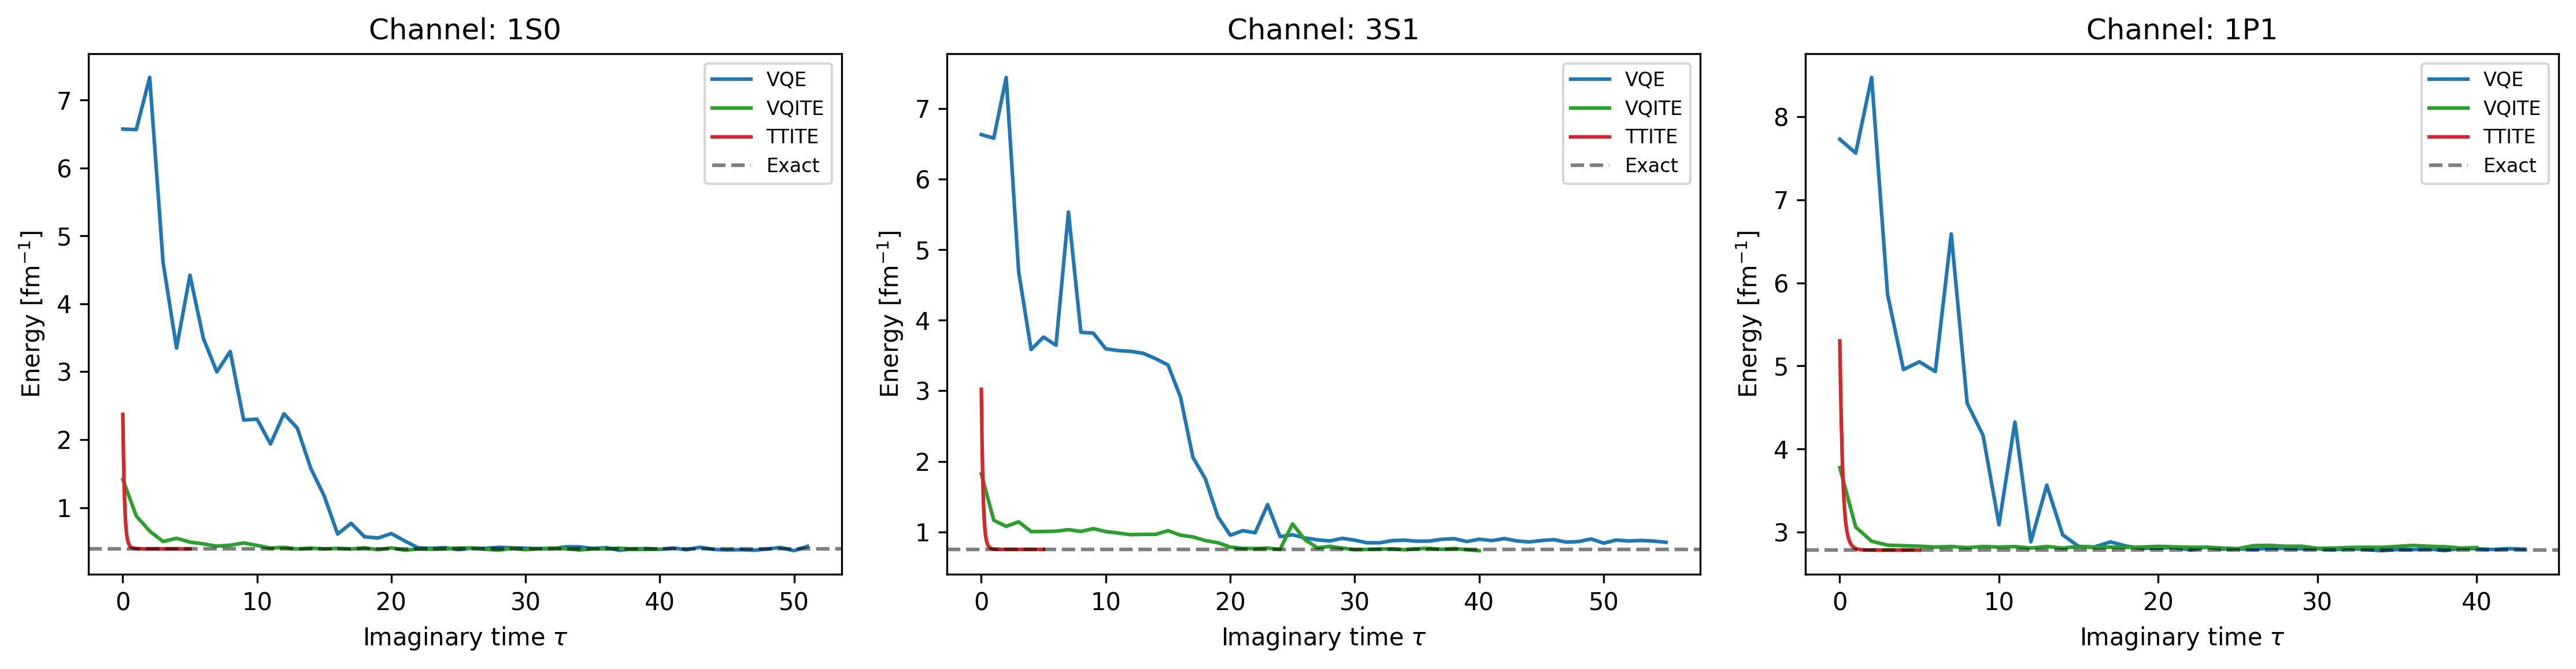
\includegraphics[width=0.85\textwidth]{convergence_comparison.png}
\caption{Convergence of each method. VQE: energy vs optimizer iteration; VQITE: energy vs imaginary-time step; TTITE: energy vs imaginary time $\\tau$.}
\label{fig:convergence}
\end{figure}



\begin{figure}[htbp]
\centering
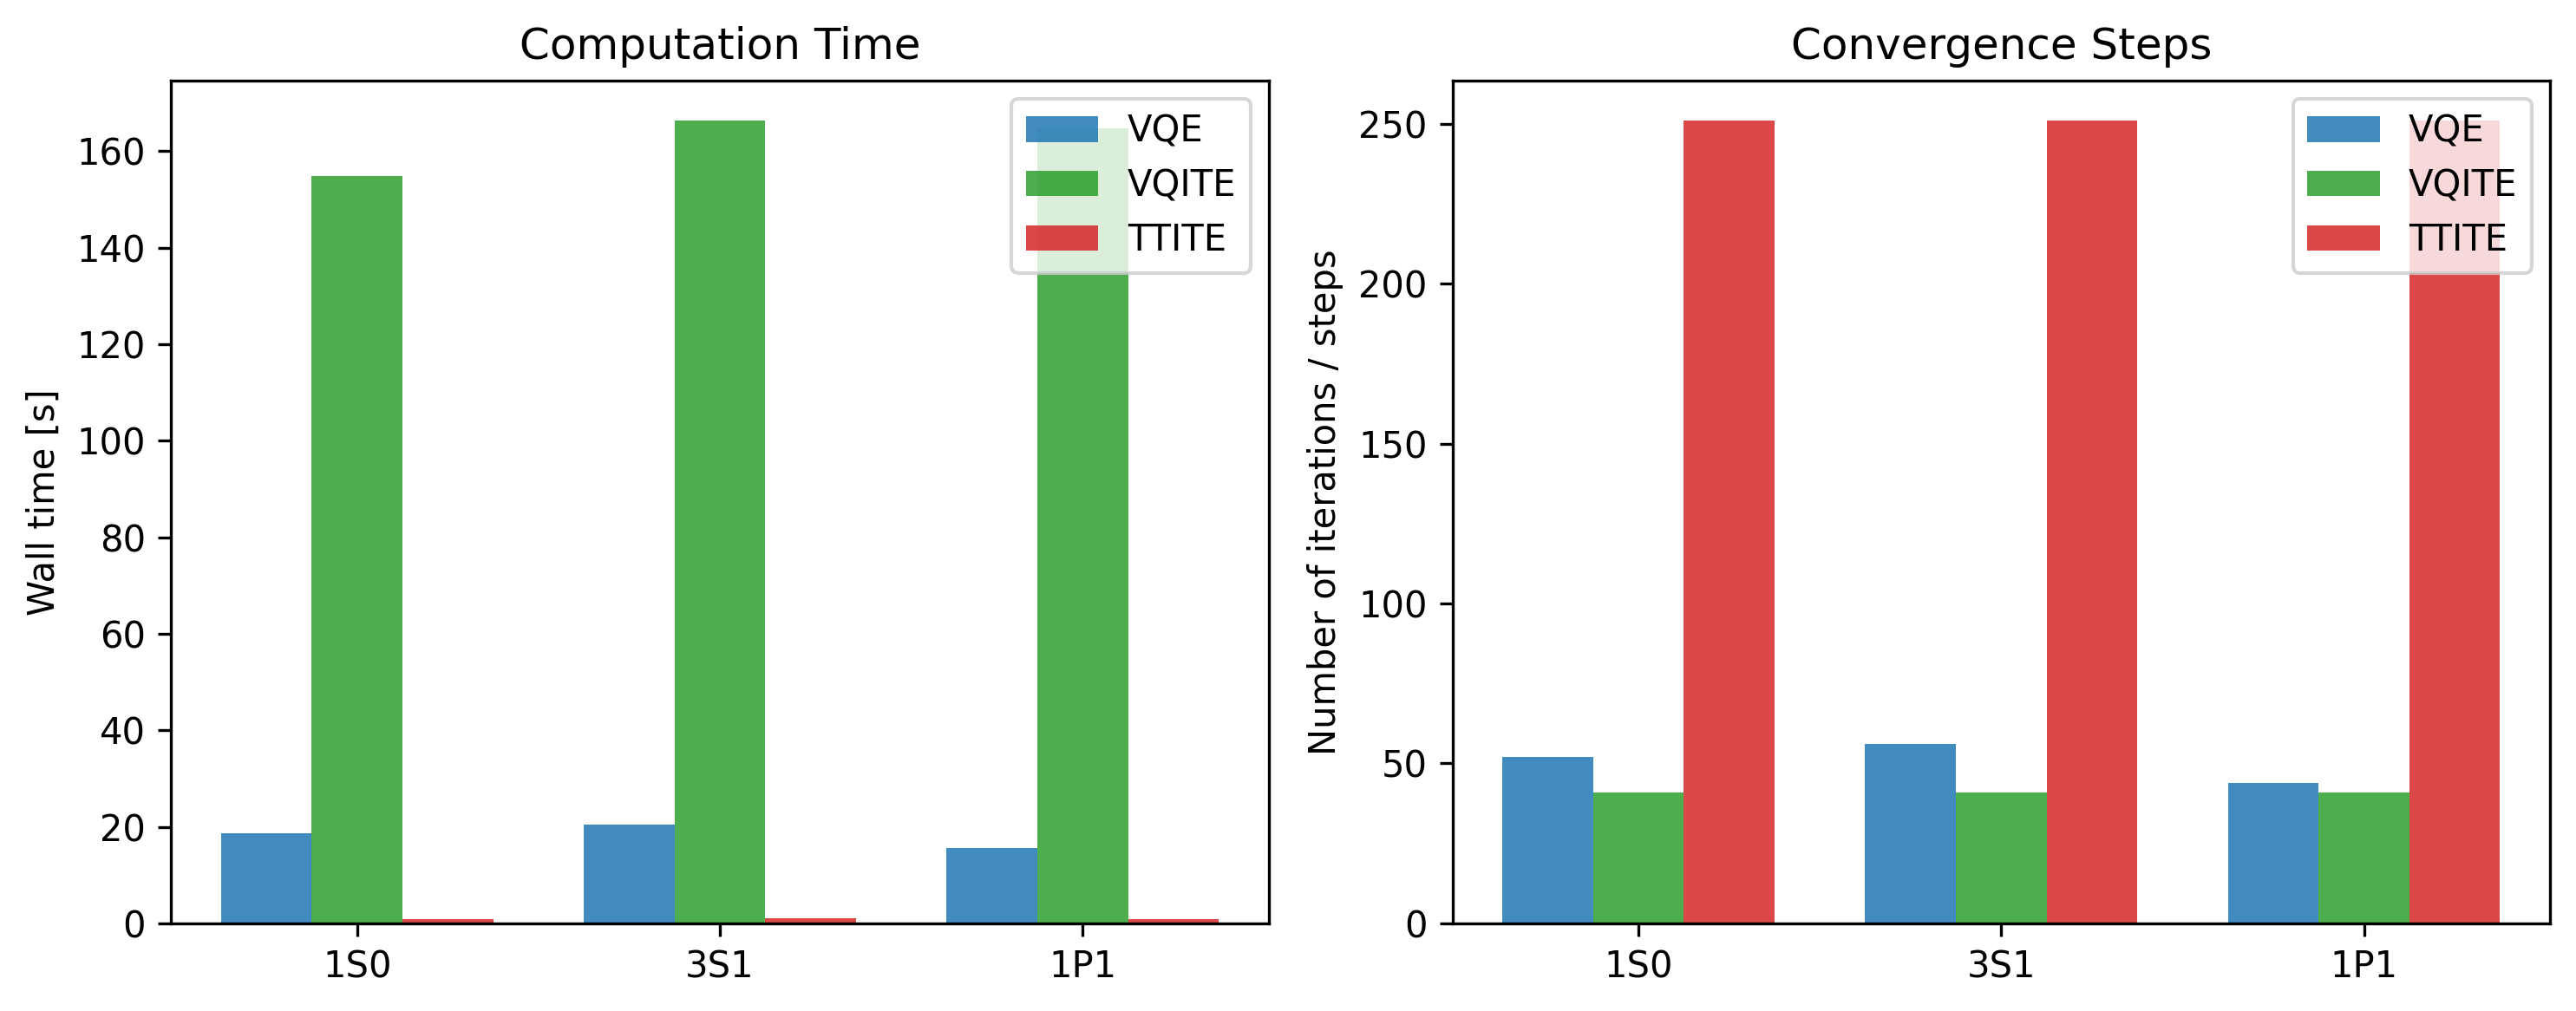
\includegraphics[width=0.85\textwidth]{circuit_cost.png}
\caption{Computation cost: wall-clock time (left) and number of iterations/steps (right).}
\label{fig:cost}
\end{figure}


%=============================================================================
\section{Excited States}
%=============================================================================

The penalty method is used for both VQE and VQITE:
\begin{equation}
  E_{\text{eff}}(\vec{\theta}) = \mel{\psi(\vec{\theta})}{H}{\psi(\vec{\theta})}
  + \alpha \sum_{j<k} \bigl|\braket{\phi_j|\psi(\vec{\theta})}\bigr|^2
\end{equation}
with $\alpha = 10$. TTITE does not support excited states.


\begin{center}
\small
\begin{tabular}{@{}l l c r r r@{}}
\toprule
Channel & Method & State & Energy & Exact & Error \\
\midrule
    1S0 & VQE & 0 & 0.4166 & 0.3913 & 0.0254 \\
    1S0 & VQE & 1 & 4.0214 & 3.4829 & 0.5386 \\
    1S0 & VQE & 2 & 4.8256 & 5.6434 & -0.8178 \\
    1S0 & VQE & 3 & 6.9489 & 7.5454 & -0.5965 \\
    \midrule
    3S1 & VQE & 0 & 0.8933 & 0.7522 & 0.1411 \\
    3S1 & VQE & 1 & 3.5227 & 3.6334 & -0.1107 \\
    3S1 & VQE & 2 & 5.6528 & 5.7265 & -0.0737 \\
    3S1 & VQE & 3 & 7.0850 & 7.6457 & -0.5607 \\
    \midrule
    1P1 & VQE & 0 & 2.7853 & 2.7813 & 0.0039 \\
    1P1 & VQE & 1 & 4.8615 & 4.8829 & -0.0214 \\
    1P1 & VQE & 2 & 8.5143 & 6.7556 & 1.7587 \\
    1P1 & VQE & 3 & 6.6872 & 8.7701 & -2.0829 \\
\bottomrule
\end{tabular}
\end{center}



\begin{figure}[htbp]
\centering
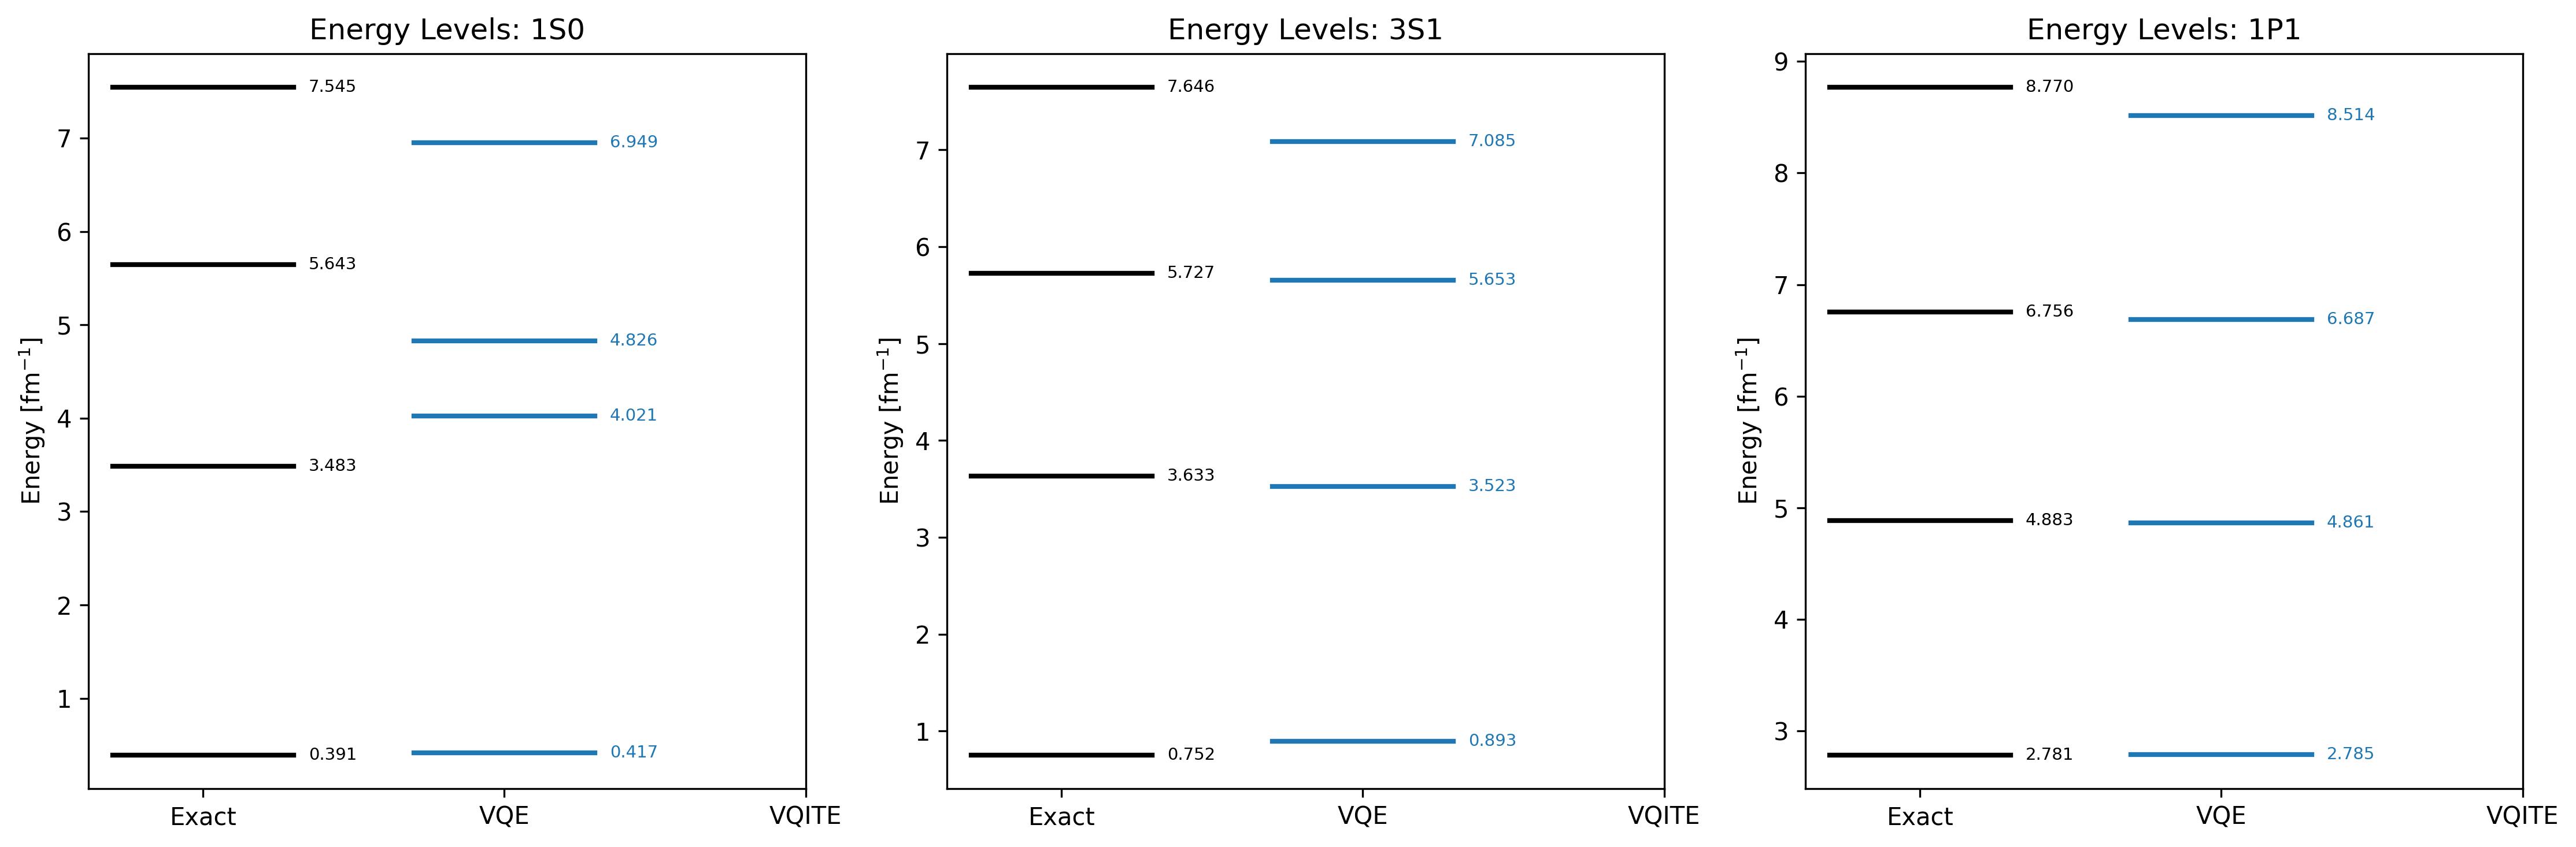
\includegraphics[width=0.85\textwidth]{excited_states.png}
\caption{Energy levels from VQE and VQITE (with penalty method) compared to exact diagonalization. TTITE finds only the ground state.}
\label{fig:excited}
\end{figure}


%=============================================================================
\section{Noise Analysis}
%=============================================================================

Each method is run under depolarizing noise at rates
$p \in \{0, 0.005, 0.01, 0.02, 0.05\}$:
\begin{itemize}[nosep]
  \item \textbf{VQE}: Shot-based measurement through noisy \texttt{AerSimulator}.
    The classical optimizer sees noisy cost function evaluations.
  \item \textbf{VQITE}: Energy gradient computed via parameter-shift rule
    with noisy shot-based measurements. Metric tensor remains statevector-based.
  \item \textbf{TTITE}: Each Trotter step applies the LCU operator followed
    by an effective depolarizing channel on the work system, modeled as
    $\rho \to (1-p_{eff})\,T_i\rho T_i^\dagger + p_{eff}\,\text{tr}(\rho)\,I/d$
    where $p_{eff}$ accounts for the gate count per step.
\end{itemize}


Representative results for channel 1S0:
\begin{center}
\small
\begin{tabular}{@{}l l r r@{}}
\toprule
Noise rate & Method & Energy [fm$^{-1}$] & Error \\
\midrule
    0.000 & VQE & $0.3836 \pm 0.0000$ & -0.0076 \\
    0.000 & VQITE & $0.3938 \pm 0.0000$ & 0.0025 \\
    0.000 & TTITE & $0.3941 \pm 0.0000$ & 0.0028 \\
    \midrule
    0.010 & VQE & $0.5146 \pm 0.0000$ & 0.1233 \\
    0.010 & VQITE & $3.2202 \pm 0.0000$ & 2.8289 \\
    0.010 & TTITE & $0.4229 \pm 0.0000$ & 0.0316 \\
    \midrule
    0.050 & VQE & $0.9358 \pm 0.0000$ & 0.5445 \\
    0.050 & VQITE & $1.2946 \pm 0.0000$ & 0.9033 \\
    0.050 & TTITE & $0.4640 \pm 0.0000$ & 0.0727 \\
\bottomrule
\end{tabular}
\end{center}



\begin{figure}[htbp]
\centering
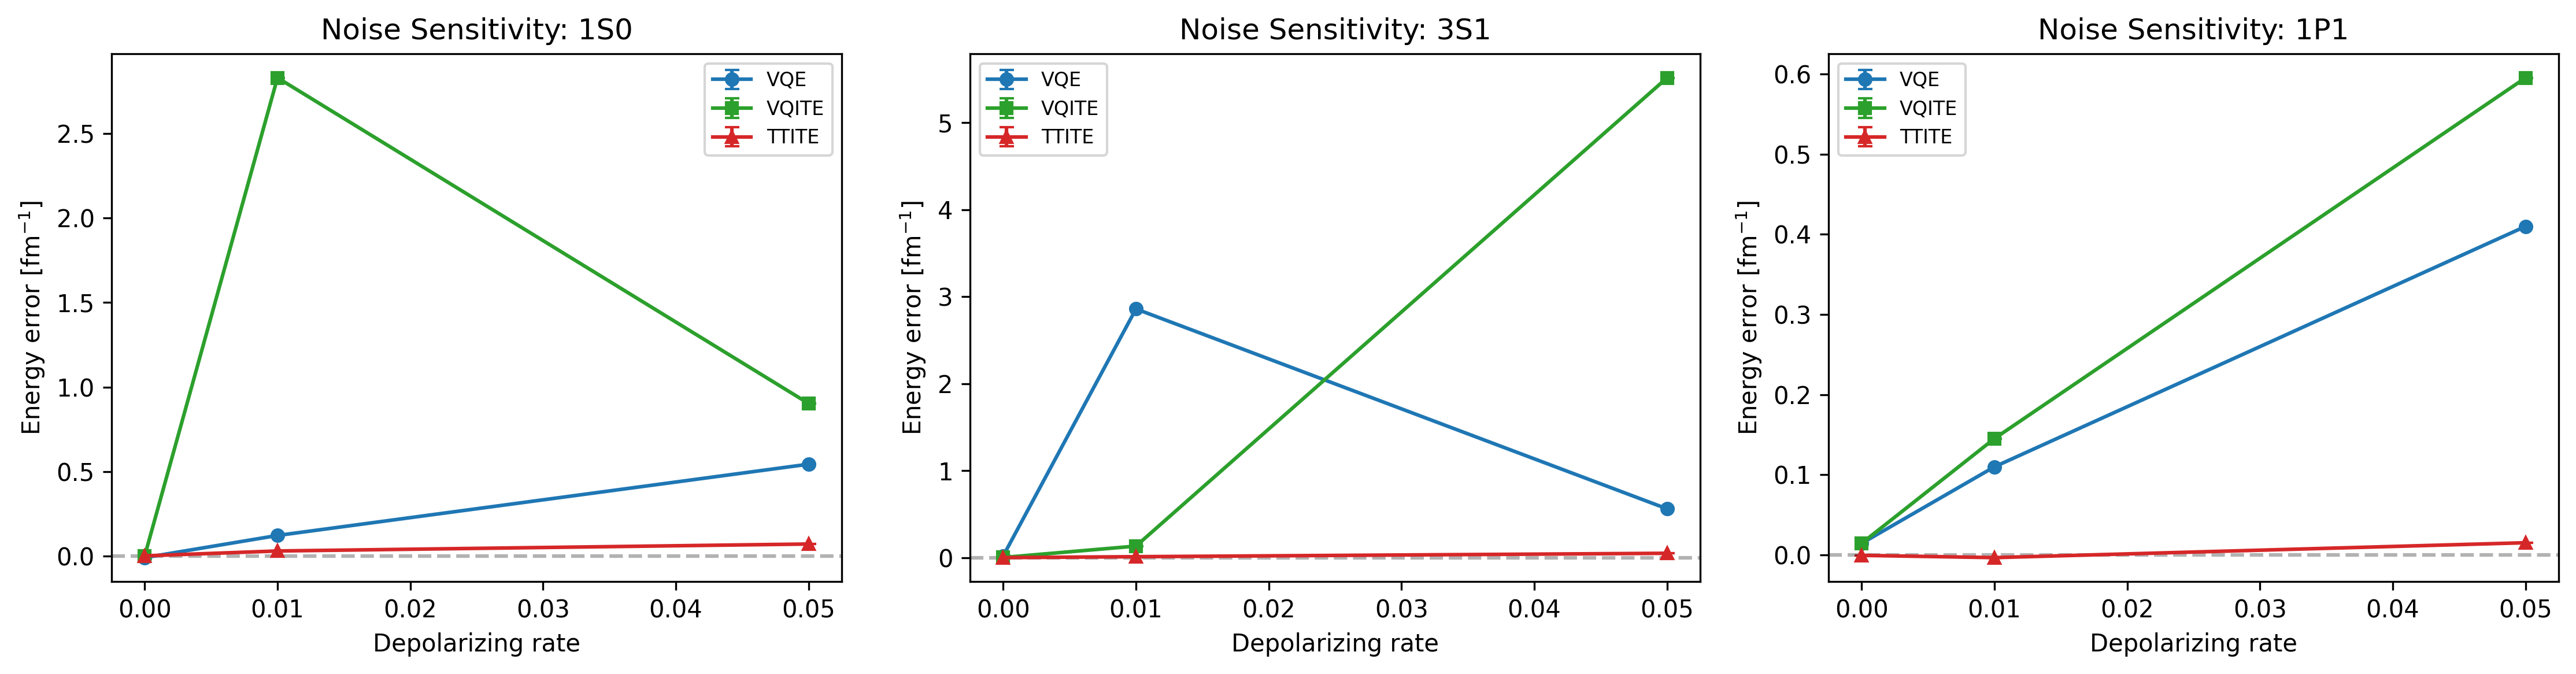
\includegraphics[width=0.85\textwidth]{noise_sweep.png}
\caption{Energy error vs depolarizing rate for all three methods. Error bars show standard deviation over repeated runs.}
\label{fig:noise}
\end{figure}



\begin{figure}[htbp]
\centering
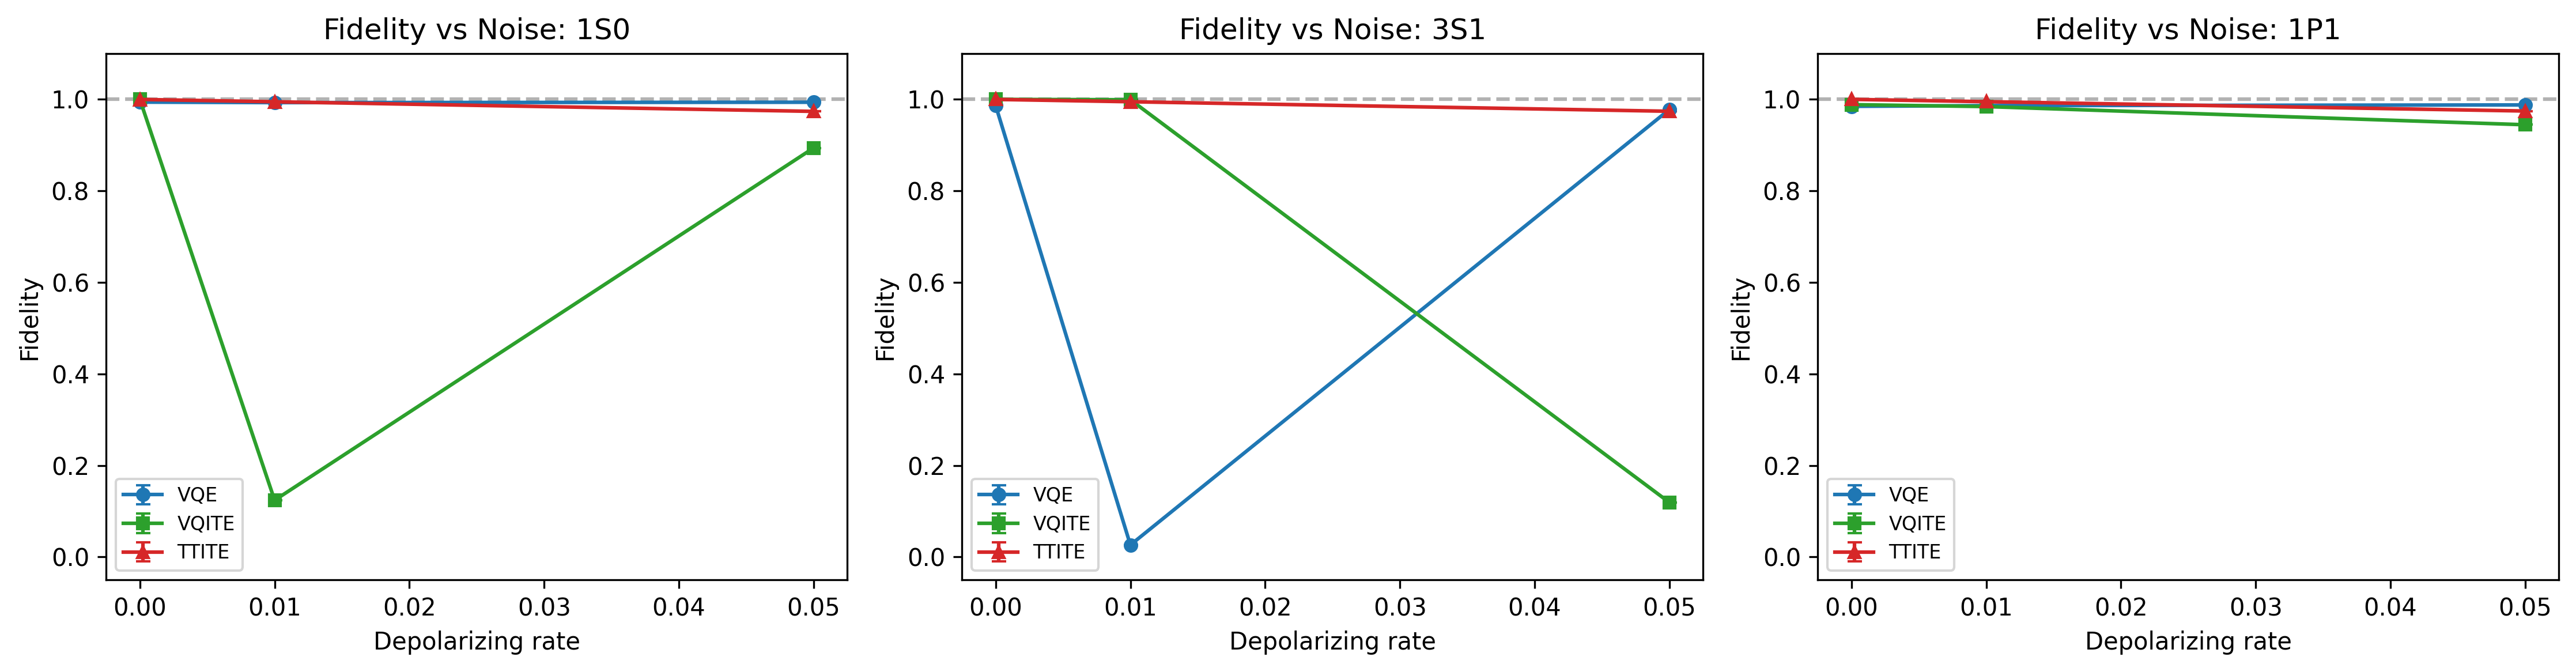
\includegraphics[width=0.85\textwidth]{fidelity_vs_noise.png}
\caption{Ground-state fidelity vs depolarizing rate.}
\label{fig:fidelity}
\end{figure}


%=============================================================================
\section{Discussion}
%=============================================================================

\subsection{Accuracy}

In the noiseless limit, all three methods converge to the exact ground-state
energy to within numerical precision. The key differences emerge under noise:
\begin{itemize}[nosep]
  \item VQE's classical optimizer can partially adapt to systematic noise,
    but shot noise limits the achievable accuracy.
  \item VQITE's natural gradient provides robust convergence even with
    noisy energy evaluations, as the metric tensor regularizes the updates.
  \item TTITE accumulates noise through its deep sequential circuit,
    with each Trotter step adding depolarization to the state.
\end{itemize}

\subsection{Convergence Speed}

VQE convergence depends on the optimizer and landscape geometry. VQITE
converges monotonically with a rate set by the spectral gap. TTITE
converges exponentially in imaginary time but requires many sequential
circuit executions.

\subsection{Practical Considerations}

\begin{center}
\begin{tabular}{@{}l c c c@{}}
\toprule
Criterion & VQE & VQITE & TTITE \\
\midrule
Ansatz required & Yes & Yes & No \\
Ancilla qubits & 0 & 0 & 1 \\
Noise resilience & Moderate & Moderate & Low \\
Excited states & Yes (penalty) & Yes (penalty) & No \\
Convergence guarantee & No & Conditional & Yes \\
\bottomrule
\end{tabular}
\end{center}

\end{document}
